% Created 2019-10-17 jue 19:04
\documentclass[presentation,aspectratio=169]{beamer}
\usepackage[utf8]{inputenc}
\usepackage[T1]{fontenc}
\usepackage{fixltx2e}
\usepackage{graphicx}
\usepackage{longtable}
\usepackage{float}
\usepackage{wrapfig}
\usepackage{rotating}
\usepackage[normalem]{ulem}
\usepackage{amsmath}
\usepackage{textcomp}
\usepackage{marvosym}
\usepackage{wasysym}
\usepackage{amssymb}
\usepackage{hyperref}
\tolerance=1000
\usepackage{khpreamble}
\usepackage{amssymb}
\DeclareMathOperator{\shift}{q}
\DeclareMathOperator{\diff}{p}
\usetheme{default}
\author{Kjartan Halvorsen}
\date{\today}
\title{Computerized Control - Polynomial design}
\hypersetup{
  pdfkeywords={},
  pdfsubject={},
  pdfcreator={Emacs 25.3.50.2 (Org mode 8.2.10)}}
\begin{document}

\maketitle


\section{Intro}
\label{sec-1}


\section{2-dof controller}
\label{sec-2}

\begin{frame}[label=sec-2-1]{Two-degree-of-freedom controller}
\begin{center}

\includegraphics[width=0.8\linewidth]{../../figures/2dof-block-explicit-no-delay}
\end{center}
\end{frame}

\section{Problem 5.3}
\label{sec-3}
\begin{frame}[label=sec-3-1]{Åström \& Wittenmark problem 5.3}
Consider the system given by the pulse-transfer function
\[ H(z) = \frac{z+0.7}{z^2 -1.8z + 0.81} \]
Use polynomial design (RST) to determine a controller such that the closed-loop system from command input to output has the characteristic polynomial
\[ A_c(z) = z^2 - 1.5z + 0.7. \]
Let the observer polynomial have as low order as possible, and place all observer poles in the origin (deadbeat observer). Consider three cases
\begin{description}
\item[{(a)}] Positional control with cancellation of the process zero
\item[{(b)}] Positional control with no cancellation of the zero
\item[{(c)}] Incremental controller with  no cancellation of the zero
\end{description}
\end{frame}

\begin{frame}[label=sec-3-2]{Why cancel the process zero?}
Bode plots of closed-loop systems (from reference signal to output) with and without cancellation of the process zero:

\begin{center}
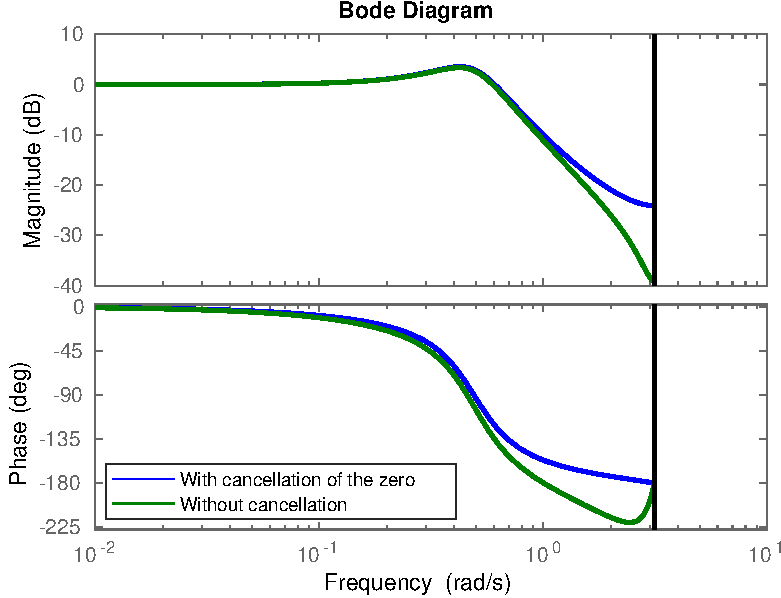
\includegraphics[width=0.6\linewidth]{../../figures/aw5_3_bode}
\end{center}
\end{frame}

\begin{frame}[label=sec-3-3]{Preliminary exercise}
Which of the closed-loop responses below  corresponds to (I) Positional control with zero cancellation (II), Positional control without zero cancellation, (III) Incremental control without zero cancellation.
\begin{center}
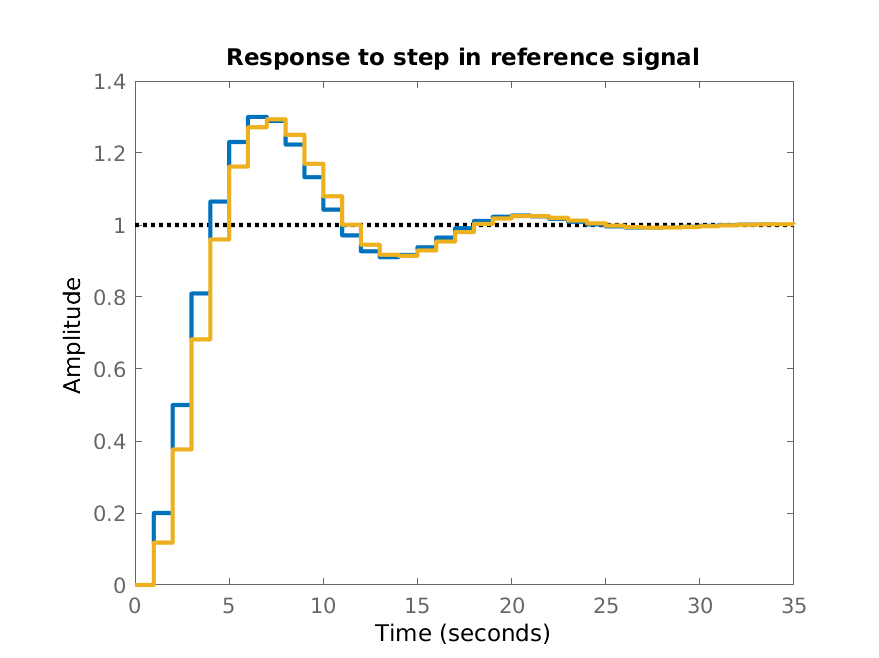
\includegraphics[width=0.45\linewidth]{../../figures/aw5_3_refstep}
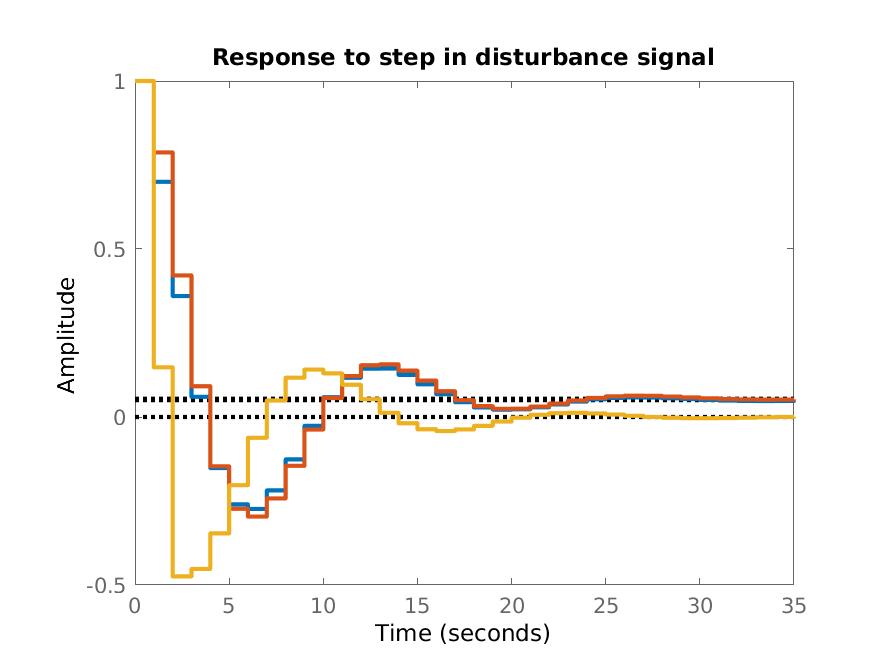
\includegraphics[width=0.45\linewidth]{../../figures/aw5_3_diststep}
\end{center}
\end{frame}
% Emacs 25.3.50.2 (Org mode 8.2.10)
\end{document}